 \chapter{Management Simulation Engine}\label{Chapter:ManagementSimulationEngine}

The hydrology of south Florida is unique due to the flat topography,
high water table, sandy soils, and high conductivity of the aquifer
system. With the rapid population growth in South Florida, the water
control system has been expanded and its operation has become
increasingly complex, making the southern Florida water management
system one of the most complex in the world.  Water levels throughout
the region are carefully regulated to minimize flood danger during wet
periods, while maximizing water supply during dry periods.  Changes in
management policies and system infrastructure are needed to address
environmental concerns, agricultural needs, changing urban water use
and flood control requirements.  A thorough investigation of the
effects of each change is required before it can be implemented.
Simulation models have become the only feasible means of assessing
system-wide impacts of the various proposed modifications to the water
resources system in south Florida.

The HSE provides a highly efficient and flexible computation engine
capable of simulating a diverse spectrum of hydrologic and hydraulic
conditions. These capabilities include the simulation of coupled
streamflow (canal) networks and ground/surface water flows, which can
be passively controlled by free-flowing structures such as weirs,
spillways, and culverts.  However, in many real world applications,
there is imposed a complex hierarchy of water resource operational
policies dependent on actuarial imposition of flow constraints on
actively controlled flow structures. To provide for simulation of such
complex, highly interrelated (coupled) water resource management
schemes within the framework of the RSM, a management module has been
carefully designed and incorporated into the RSM.

The Management Simulation Engine (MSE) consists of a multi-level
hierarchical control scheme, which naturally encompasses the local
control of hydraulic structures, as well as the coordinated
sub-regional and regional control of multiple structures. MSE
emphasizes the decoupling of hydrologic state information from the
managerial decision algorithms, facilitating the interoperation and
compatibility of diverse management algorithms and providing
flexibility to adapt a model implementation to swiftly changing
operational policies on the ground. The MSE is intended to allow a
flexible, extensible expression of a wide variety of anthropogenic
water resource control schemes integrated with the hydrologic state
evaluations of the RSM. Synergy between the multilayer control
hierarchy and decoupled hydrologic state and management information
facilitates a water resource management feature set not typical of
integrated hydrologic models.  The MSE design is based on the
principle that operational and managerial decisions applied to water
control structures can be viewed as information processing algorithms
decoupled from the hydrologic state information on which they
operate. Essentially, the HSE provides hydrologic and hydraulic state
information, while external policies that dictate managerial
constraints and objectives are applied through MSE controllers and
supervisors.

In cases where discrete spatiotemporal model inputs are sufficient for
controller and supervisor algorithms, the MSE accepts inputs directly
from HSE data monitors. However, in cases where integrated
spatiotemporal state information, or aggregated state information
based on specific pre-processing is required, the MSE is able to store
and access information in the MSE Network.  

The MSE network is an abstraction of reservoirs, streams and canals
(water bodies), together with a stream/canal flow network and water
control structures (water movers) dedicated to representing the
managerial architecture of the model.

MSE is an integral component of the RSM, and provides two modes of
functionality in the analysis and prediction of water control
structure operational behaviors:

\begin{enumerate}
 \item Simulate existing water resource policies through assessment of
   currently implemented management operational policies and rules in
   response to hydrologic forcing (e.g., rain, ET)
 \item Develop alternative resource control strategies through the
   optimization of operational policies and rules
\end{enumerate}

The first mode is a critical capability for the assessment of water
control operations in response to historic, real-time, or forecast
forcing conditions. The second mode forms an important analysis tool
aimed at identification of alternative operational policies which must
perform complex, multi-variate, resource allocation functions under
the control of system boundary conditions and constraints. The MSE is
formulated to address both of these needs by incorporating a variety
of supervisory control algorithms including rule-based expert systems,
finite state-machine processors, as well as a generic mathematical
programming language interface, which provides access to a suite of
state-of-the-art optimization algorithms (Park et al.,
2007)\nocite{Park:2007}.

The MSE is therefore capable of addressing specific water resource
allocation analysis, for example:

\begin{itemize}
 \item Enable water resource reallocation in response to competing
   demands during a water shortage 
 \item Diminish flow/containment problems during flood situations
 \item Consider downstream needs for water supply
\end{itemize}

From a functional perspective, the MSE is essentially an information
filter tasked with the imposition of flow constraints on model water
control structures. This is accomplished within the framework of the
RSM in three coupled operations: data gathering, data processing and
decision making, and decision application, as represented in Figure
\ref{Fig:mseFunctions}. An overview of each of these areas relevant
to their implementation in the MSE is discussed in the following
sections.

\begin{figure}
 \begin{center}
  
\includegraphics[scale=.85]{Graphics/mseFunctions.eps}
 \end{center}
 \caption{\label{Fig:mseFunctions} Functions of the Management Simulation Engine.}        
\end{figure}

\section{Information Gathering from HSE}

All hydrologic and hydraulic state information including water stages,
flow values, rainfall, ET, hydrologic boundary conditions, or any
other state variable used as input or computed as output by the HSE is
available to the MSE and the assessors through the implementation of a
uniform data monitor interface. The data monitor interface extends
naturally to the MSE input/output variables. Therefore, the input
state information available to a controller or a supervisor is not
limited to water levels or flow values, but can include control
information, decision variables, constraints or any other management
variable from any other assessor or supervisor in the model.  

A central feature of the MSE, which enables decoupling of the
hydrologic state information maintained by the HSE and the operational
process information of the MSE, is the MSE network (Figure
\ref{Fig:mseNetwork}).  This network is based on a standard graph
theory representation of a flow network comprised of arcs and nodes
(Ahuja et al., 1993; Ford and Fulkerson,
1962)\nocite{Ahuja:93}\nocite{Ford:62}.

\begin{figure}
 \begin{center}
  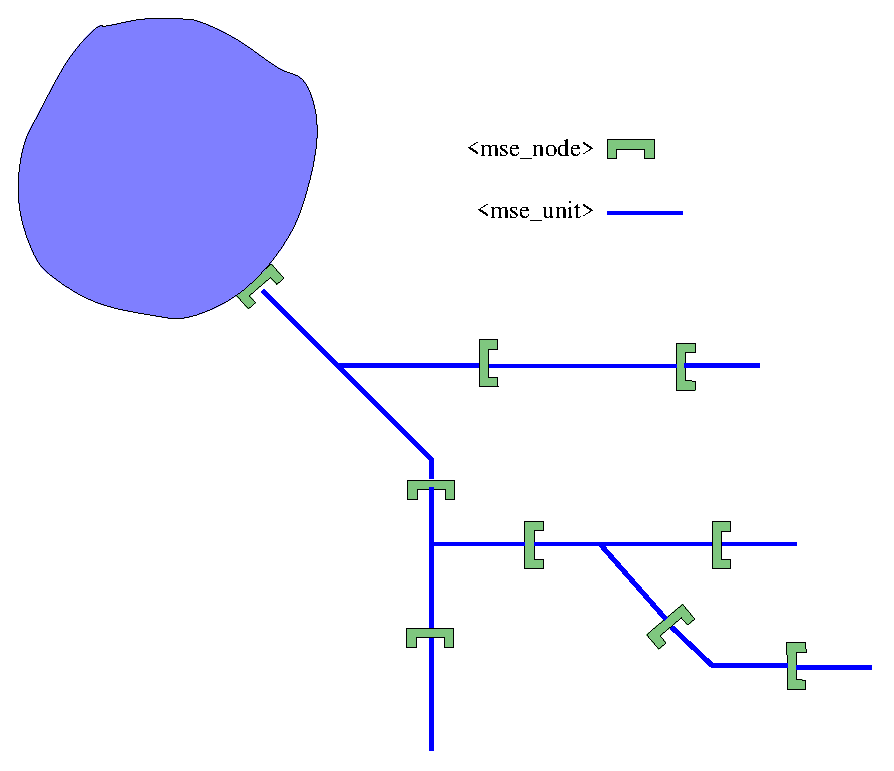
\includegraphics[scale=0.5]{Graphics/mseNetwork.eps}
 \end{center}
 \caption{\label{Fig:mseNetwork} The MSE network structure}        
\end{figure}

From the hydrologic perspective, the HSE canal network is composed of
an interconnected network of segments, with each segment maintaining
parameters relevant to aquifer stream interaction, flow resistance,
spatial coordinates and other physical properties (Figure
\ref{fig:hseNetwork}). The spatial representation of HSE segments is
typically dictated by topographic and physical parameters. From the
water resource management viewpoint of the MSE, the important features
of the flow network are its connectivity, flow capacities, flow
regulation structures, and assessed state information relevant to
managed sections of the network. 

\begin{figure}
 \begin{center}
  
\includegraphics[scale=0.75]{Graphics/hseNetwork.eps}
 \end{center}
 \caption{\label{fig:hseNetwork} The HSE network structure}        
\end{figure}

The primary data object in the MSE network is the water control unit
(WCU). A WCU maps a collection of HSE water bodies that are
operationally managed as a discrete entity in the MSE network. WCUs
are typically bounded by hydraulic control structures, which are
represented as nodes in the MSE network. Each WCU includes associative
references to all inlet and outlet hydraulic flow nodes.

The MSE network data objects serve as state and process information
repositories for management processes. They maintain assessed and
filtered state information, provide parameter storage relevant to a
water control unit (WCU) or hydraulic structure managerial constraints
and variables, and serve as an integrated data source for any MSE
algorithm seeking current state information. Some variables stored in
a structure (node) object include:

\begin{itemize}
 \item current flow capacity of a physical structure
 \item maximum design flow capacity of a physical structure
 \item reference to hydraulic watermover(s) in HSE
 \item reference to structure controller(s) in MSE
 \item operational policy/rule water levels
 \item water supply
 \item water demands
\end{itemize}

The WCU objects incorporate:
\begin{itemize}
 \item time-varying or seasonal stage maintenance levels
 \item flood control stage maintenance levels
 \item inlet flow
 \item outlet flow
 \item water volume
\end{itemize}

Each WCU in the MSE network is referenced by a unique label, and has
an associative data storage object which dynamically allocates storage
for assessment results. This allows multiple, independent assessments
of the WCU state. For example, one assessment of WCU inlet structure
flows might come from a graph algorithm, while another could be
obtained from a LP model.

This abstraction from hydrologic objects to managerial objects
condenses the network representation facilitating the organization and
storage of relevant assessed state and process information. As an
example, Figure \ref{fig:hseNetwork} depicts an HSE canal network
consisting of 63 nodes and 62 segments. Some of the nodes correspond
to locations of hydraulic control structures, though the association
is not apparent from examination of the HSE network. Each canal
segment has a unique identifier which allows the modeler or MSE
processor to monitor state information of the segment. However, it may
be appropriate to make water management decisions based on some
assessed or filtered version of aggregated canal segment states.
Consider now an abstraction of the HSE network into 10 WCUs, regulated
by 11 hydraulic structures, as shown in Figure
\ref{Fig:mseNetwork}. In the MSE network each line segment represents
a WCU, while each node represents a hydraulic structure which
regulates a WCU. The modeler or MSE processor is able to directly
monitor information stored in any of these object data containers,
information which has already been assessed and automatically stored
in the appropriate WCU data object at each timestep.  As with other
RSM model inputs, the WCU mapping from the HSE canal network is
performed with an input XML entry.

The MSE network can also be mapped to basin scale implementations of
the HSE, where regional hydrologic system is simulated by an
interconnected network of basins and lakes, and hydrologic stressors
are applied directly to the basins and lakes through boundary
conditions, rainfall, and ET. The routing of water in the regional
system is governed through operational management policies imposed by
the MSE.  Basin scale implementations have the same important network
flow features (connectivity, flow capacity, etc) as their more complex
distributed mesh/network counterparts.  Water control units are mapped
to basins and lakes and the nodes are mapped to the structures that
provide connectivity between the basins and lakes.

\section{Decision Making: Supervisors, Assessors}

The MSE architecture is based on a multilayered hierarchy, with
individual water control structures regulated by controllers while the
regional coordination and interoperation of controllers is imposed by
supervisors. Supervisors can change the functional behavior of
controllers, completely switch control algorithms for a structure, or
override the controller output based on integrated state information
and/or rules. A schematic depiction of the HSE-MSE layered hierarchy
is shown in Figure \ref{fig:multiLayerHierarchy}.  

\begin{figure}
 \begin{center}
  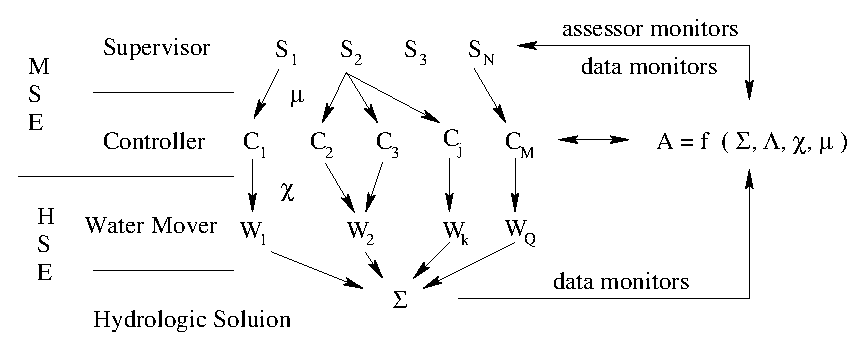
\includegraphics[scale=.85]{Graphics/multiLayerHierarchy.eps}
 \end{center}
 \caption{\label{fig:multiLayerHierarchy} RSM multilayer control hierarchy.}
\end{figure}

At the lowest layer is the hydrologic state information ($\Sigma$)
computed by the HSE. This information includes water stages, flow
values, rainfall, ET, hydrologic boundary conditions, or any other
state variable used as input or computed as output by the HSE. All
such variables are made available to the MSE and assessors through the
implementation of a uniform data monitor interface. This transparency
of state and process information throughout the model is central to
the efficient synthesis and processing of heterogeneous information
required to simplify and naturally express complex water management
policies.  The top level of the MSE is the supervisory layer. There is
no limit on the number of supervisory algorithms, or constraint on the
number of controllers that a supervisor may influence. Based on state
and process information, which optionally may have been filtered or
assessed, the function of a supervisor is to produce the supervisory
control signal ($\mu$) for a single, or collection of, hydraulic
structure controllers. The supervisors are therefore able to
comprehensively coordinate the global behavior of multiple independent
or coupled hydraulic structures.

\subsection{MSE Supervisors}
An MSE supervisor is effectively a meta-controller, a controller of
controllers. The addition of this supervisory layer considerably
simplifies the control expression of multiple, coordinated hydraulic
structures. In addition to the organizational simplification of
control algorithms, the additional layer enables representation of
management functions which are not realizable with a single control
layer.

In relation to the controllers, which are multi-input single-output
(MISO) processors, the supervisors are multi-input multi-output (MIMO)
processors. Supervisors have the ability to change individual response
characteristics of controllers, or, in the case of multiple
controllers attached to a watermover, to dynamically select and
activate a specific controller for any watermover. Specifically, the
supervisory functions include:

\begin{itemize}
 \item Comprehensive assessment of state and process information
 \item Controlling multiple parameters of multiple controllers
 \item Dynamic switching of multiple controllers
 \item Flow regulation override for controller(s)
\end{itemize}

Supervisors can therefore change the functional behavior of
controllers, completely switch control algorithms for a structure, or
override a controller output based on integrated state information
and/or rules.

There is no practical limit on the number of supervisors allowed in a
model, or on the number of controllers that a supervisor may
affect. It is common to have a hybrid selection of different
supervisors, each one regulating a specific sub-regional collection of
hydraulic structures. The ability to selectively tailor management
control algorithms, as well as the flexibility to easily reconfigure
them in a plug-and-play fashion lends considerable power to the
implementation of diverse and complex operational management
scenarios.  The current suite of supervisors includes:

\begin{itemize}
 \item Fuzzy rule based
 \item GLPK Linear Programming (GNU Linear Programming Kit)
 \item Finite state machine (user defined)
 \item Heuristic assessors to capture special operations for a
   particular modeled area
\end{itemize}

These supervisors are discussed in more detail in South Florida Water
Management District (2005) \nocite{sfwmda:2005}.

\subsection{Assessors and Filters}
In the RSM, state and process information can be functionally
transformed by an independent set of filters, which can be viewed as
information pre-processors. These processors are denoted as assessors
and filters. For example, an assessor may perform statistical
filtering such as spatiotemporal expectations, amplitude or time-delay
modulation, or any other suitable data filtering operation. The MSE is
then tasked with appropriately processing the assessed state
information to produce water management control signals, which are
applied to the hydraulic control structures to satisfy the desired
constraints and objectives.  

The role of assessors in the MSE is to perform data preprocessing
required for operational control decisions. By decoupling the
conditioning and filtering of state and process information from the
decision making algorithms, the decision processors can be simplified
and modularized. Therefore, an assessor is an information processor
intended to provide specialized aggregation or differentiation of
state variables particular to a managerial decision process. The suite
of assessors provides for specialized quantification of hydrologic
state variables freeing managerial algorithms from data preprocessing.

Related to the assessors are MSE filters. Filters are generic
information processors implemented to perform simple, often redundant
data filtering operations. The RSM implements a unified design
approach and interface for monitors, filters, and assessors based on
object oriented design principles. As a result, the interfacing of
these constructs from the users perspective is particularly simple and
powerful. Assessor, filters and monitors can operate in a piped FIFO
(first-in, first-out) fashion.

\section{Imposition of Decisions on HSE: Controllers}
The MSE controllers are the intermediary between the hydraulic
structures (watermovers) and the regional-scale supervisory
coordinators. The controllers can operate independently of the
supervisors; in fact, they are not required at all for uncontrolled
operation of a hydraulic structure (e.g., an uncontrolled
spillway). The essential purpose of a controller is to regulate the
maximum available flow through a structure to satisfy a local
constraint. A controller may take as an input variable any state or
process information which can be monitored within the RSM. Since the
interface between a structure watermover and any controller is
uniform, it is possible to change controllers dynamically with a
supervisory command, or manually with a simple XML input change. The
unitary interface also allows for the modeler to mix and match
controllers in a particular model application so that the local
control schemes are a hybridization of any of the available control
algorithms.

At each model time step, once the controllers have computed their
respective control values, these signals are applied as flow
constraints to the structure watermovers in the HSE. Each watermover
will compute a maximum flow capacity based on the hydrologic state
conditions and hydraulic transfer function of the structure. The
resultant controlled flow will be some fraction of the currently
available maximum flow capacity. 

